% Abbreviations: EEE, ACS, PCB.

\documentclass{article}
\usepackage{graphicx}
\usepackage{textcomp}
\usepackage{eurosym}
\usepackage{rotating}
\graphicspath{{./images/}}
\title{Project Plan}

\begin{document}
\maketitle
\section{Planning}
For many project, it can be a challenge to oversee all activities that need to be completed. 
To manage the activities for this project, a Gantt Chart was made, which can be found in Appendix A.
When creating the Gantt Chart, activities found in Chapter 3 were kept in mind.
The Gantt Chart is divided in three sections: tasks everyone works on, tasks specific to EEE students, and tasks specific to ACS students.
Besided activities, the Gantt Chart also contains several milestones.

\section{Costs and Benefits}
\subsection*{Employees}
The team consists of six people, of which two EEE students, and four ACS students.
According to the website of Saxion, the starting salary of an EEE graduate working 38 hours a week \euro{}3.071,-, and for an ACS graduate working 36 hour weeks this will be \euro{}2.860,-.
An approximation can be made that employees with an EEE related position earn \euro{}20,20 an hour while software engineers have an hourly salary of \euro{}19,60.
The workload for this project is thirteen hours a week during the third quarter and sixteen hours a week as of the fourth quarter.
Both quarters contain eight working weeks, which means that the total workload will be 232 hours per team member.
With this information, it can be concluded that approximately \euro{}27.561,60 has to be spend on salaries.

\subsection*{Hardware}
A 3D printer may be utilized for this project, but since it's not clear if this has a use case for our product, the costs for this aren't taken in consideration yet.
Add more text if we roughly know what components we need to use.

\subsection*{Software}
At this stage of the project it's difficult to say what software will be used for developing the final product but for the costs an estimation can be made.
When designing the PCB, a licence might be needed depending on the program being used for doing so.
The team works with various Microsoft 365 products such as: Word, PowerPoint, and OneDrive.
As of today, a standard licence for these products costs \euro{}11,70 a month. 
The team consists of six people so \textup{\euro}70,20 has to be spend a month.
The project takes approximately four months, this means that in total \euro{}280,80 has to be spend on Microsoft 365 licences.

Depending on what tools will be used for writing the software, there's a chance that there will be costs for licences.
Assuming the microcontroller used in the final product is an ESP32 or something similar, it can be concluded that this won't result in extra costs since there are plenty of free resources available for programming such devices.

\begin{table}[htbp]
\centering
\caption{Costs}
\begin{tabular}{c|c|c|c}
Employees & Hardware & Software & Total \\
\hline
\euro{}27.561,60 & ? & \euro{}280,80 & ? \\
\end{tabular}
\end{table}
\newpage

\begin{sideways}
\centering
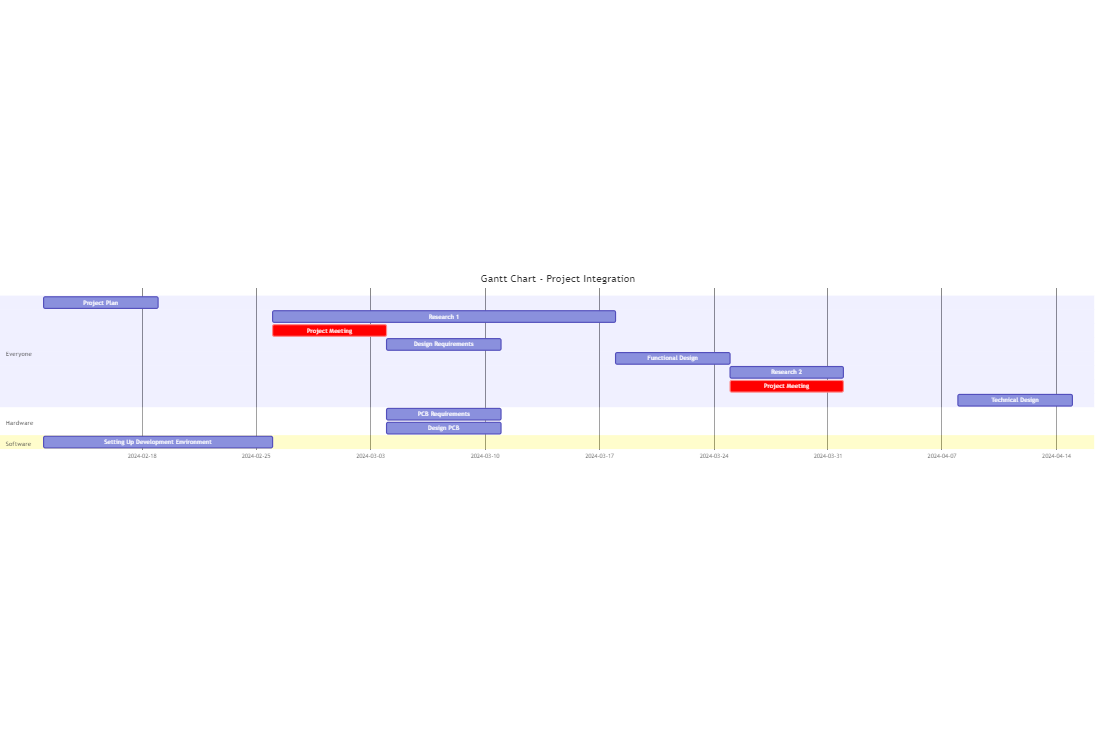
\includegraphics[width=\paperheight]{images/gantt-chart.png}
\end{sideways}

\end{document}
